\section{Etapa de decodificaci\'on}

En esta etapa, mediante la obtenci\'on de la instrucci\'on a trav\'es del latch entre esta etapa y la etapa de b\'usqueda de la instrucci\'on, se procede a activar señales y separar los datos para que se ejecute la instrucci\'on proporcionada de manera correcta.
Las entradas a esta etapa se pueden ver en la figura \ref{fig:decode}.

\begin{figure}[H]
\centering
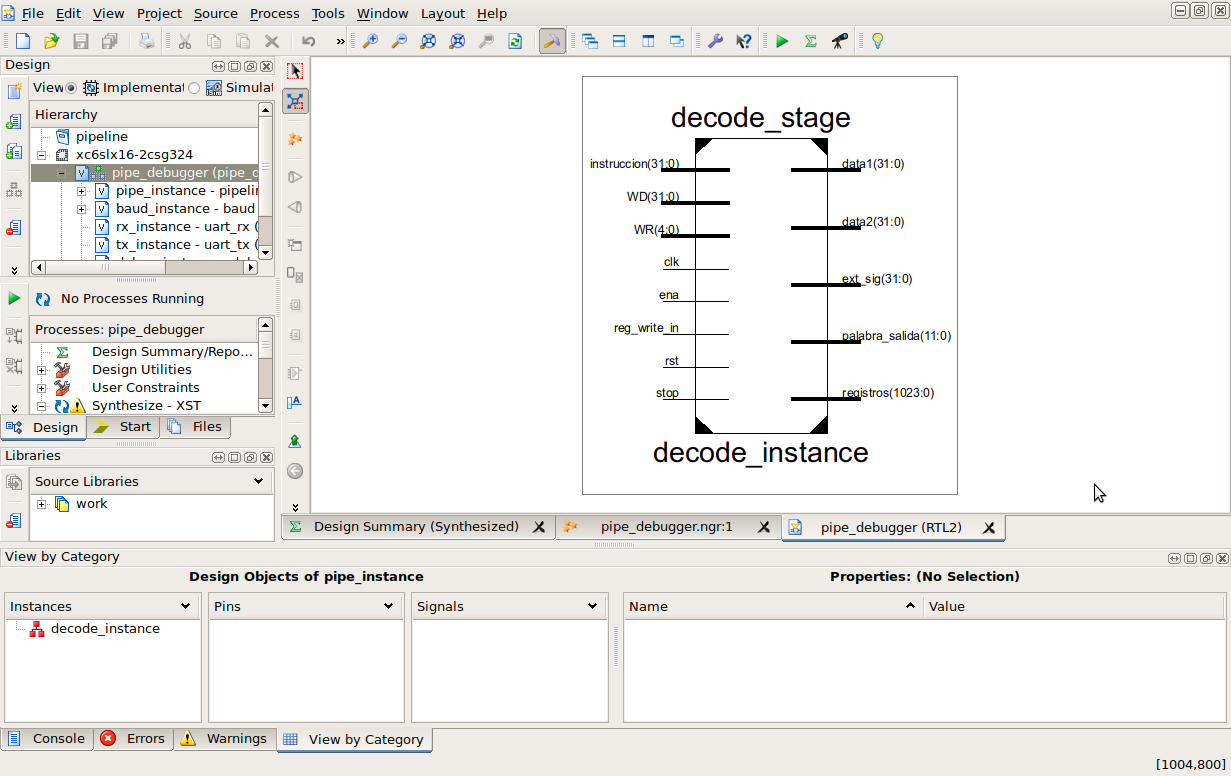
\includegraphics[scale=0.5]{img/decode_stage}
\caption{Etapa de decodificaci\'on}
\label{fig:decode}
\end{figure}

 
Las entradas son: 
\begin{itemize}
  \item \textbf{instruccion}: Bus de 31 bits de ancho que contiene todo lo necesario para que se ejecute la etapa de decodificaci\'on.
  \item \textbf{WD}: Datos que se van a escribir en el banco de registros en WR.
  \item \textbf{WR}: Registro que se va a escribir el dato WD.
  \item \textbf{clk}: Clock general del sistema.
  \item \textbf{ena}: Señal de habilitaci\'on del m\'odulo.
  \item \textbf{reg\_write\_in}: Señal que habilita la escritura de un registro del banco de registros.
  \item \textbf{stop}: Señal que para la ejecuci\'on y el funcionamiento normal del m\'odulo en caso de que exista alg\'un branch o jump. 
\end{itemize}

Esta etapa contiene m\'odulos que son fundamentales para su funcionamiento, la etapa m\'as en detalle se puede ver en la figura \ref{fig:decodedetail}, estos m\'odulos son la unidad de control, el banco de registros, la unidad de extensi\'on de signo y un multiplexor.

\begin{figure}[H]
\centering
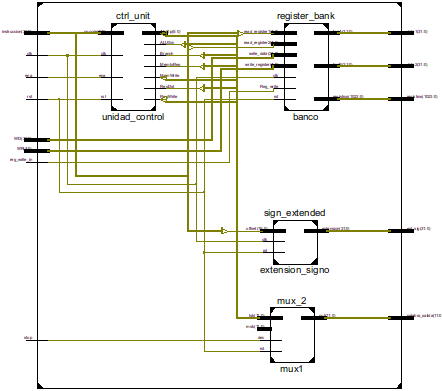
\includegraphics[scale=0.7]{img/decode_stage_inside}
\caption{Detalle etapa de decodificaci\'on}
\label{fig:decodedetail}
\end{figure} 

\subsection{Unidad de control}
La unidad de control se encarga de tomar la parte mas alta de la palabra y decodificar el tipo de instrucci\'on (ver figura \ref{fig:ctrl_unit}) para activar o desactivar señales que se encargan de activar o desactivar multiplexores y otros m\'odulos.

\begin{figure}[H]
\centering
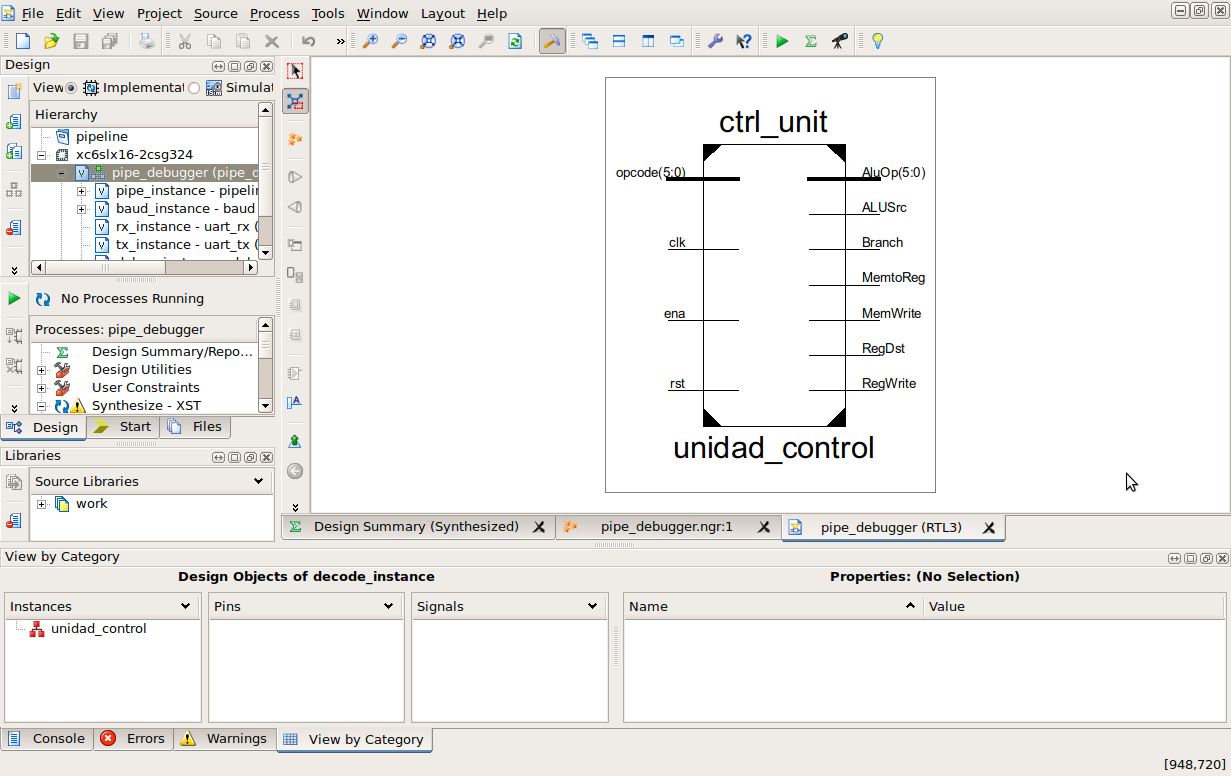
\includegraphics[scale=0.5]{img/unidad_control}
\caption{Unidad de control}
\label{fig:ctrl_unit}
\end{figure} 

Tiene como entradas:
\begin{itemize}
  \item \textbf{opcode}: Bus de 6 bits que es la parte alta de la instrucci\'on.
  \item \textbf{clk}: Clock general del sistema.
  \item \textbf{ena}: Entrada de habilitaci\'on del chip.
  \item \textbf{rst}: Entrada de reset del chip.
\end{itemize}

Y las salidas:
\begin{itemize}
  \item \textbf{aluOp}: Bus de 6 bits que llega a la etapa de ejecuci\'on, pasando antes por el latch hacia la unidad de control de la alu, que sirve para decirle a la alu que operaci\'on l\'ogica realizar.
  \item \textbf{aluSrc}: Cable que va a un multiplexor en la etapa de ejecuci\'on que elige que tipo de dato va a entrar a la alu.
  \item \textbf{Branch}: Señal que se activa en caso de que alg\'un salto sea detectado.
  \item \textbf{MemtoReg}: Señal que se activa en caso de que se deban mover datos de memoria hacia registros.
  \item \textbf{MemWrite}: Señal que se activa en caso de que se vaya a escribir en la memoria de datos.
  \item \textbf{RegDst}: Señal que se activa y llega a un multiplexor para decidir que registro se va a elegir para escribir.
  \item \textbf{RegWrite}: Señal que entra en el banco de registros y le indica si debe o no escribir alguno de los 32 registros que posee. 	
\end{itemize}

\subsection{Banco de registros}
El banco de registros es el m\'odulo que se encarga de guardar las variables que el usuario usa para los programas, pueden ser escritos directamente o desde memoria. La figura \ref{fig:registros}muestra en detalle este m\'odulo.

\begin{figure}[H]
\centering
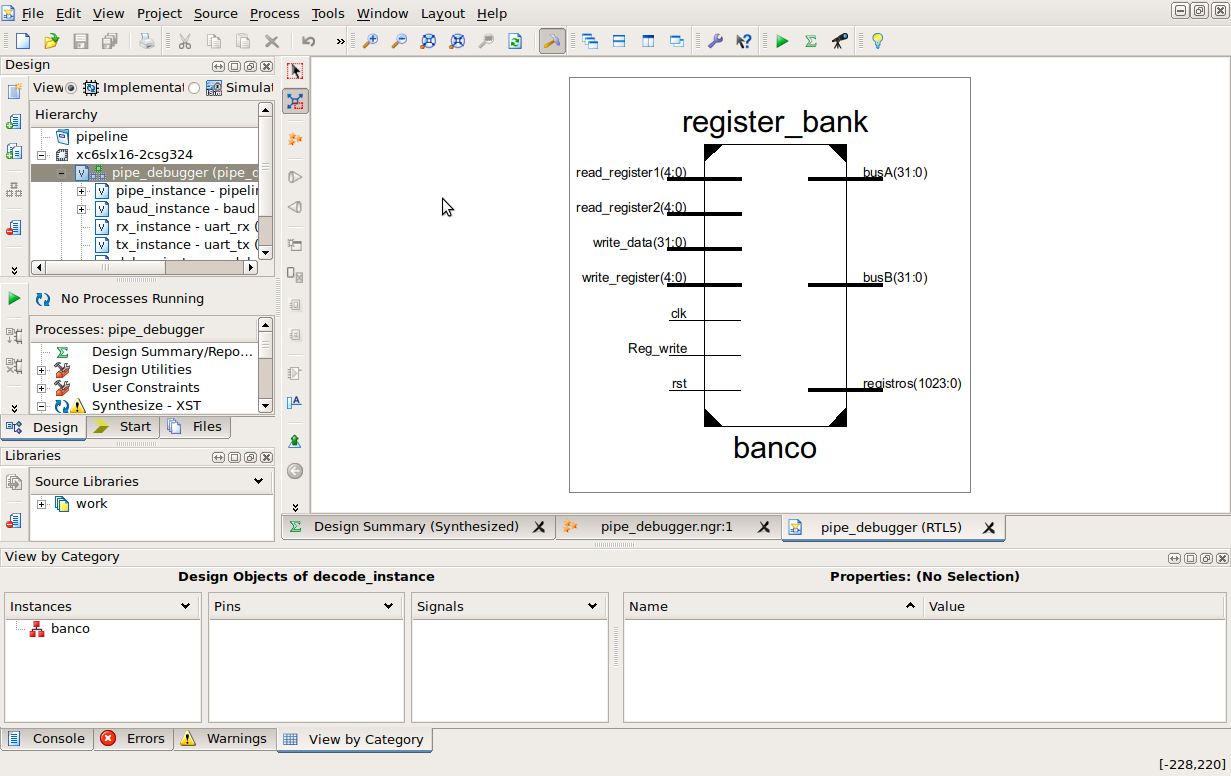
\includegraphics[scale=0.5]{img/banco_registros}
\caption{Banco de registros}
\label{fig:registros}
\end{figure} 

Tiene como entradas:
\begin{itemize}
  \item \textbf{read\_register1}: Bus de 5 bits que indica que registro leer.
  \item \textbf{read\_register2}: Bus de 5 bits que indica que registro leer.
  \item \textbf{write\_data}: Bus de 32 bits que contiene el dato que se va a escribir en el registro si es que est\'a habilitada la senal de escritura de registros (RegWrite).
  \item \textbf{write\_register}: Bus de 5 bits que indica que registro se va a escribir en caso de que est\'e habilitada la señal de RegWrite de la unidad de control.
  \item \textbf{Reg\_write}: Señal que habilita la escritura de un registro del banco de registros.
  \item \textbf{clk}: Clock general del sistema.
  \item \textbf{rst}: Reset del banco que coloca todos los valores de los registros a 0.  
\end{itemize}

Las salidas son:
\begin{itemize}
  \item \textbf{busA}: Bus de 32 bits que da el valor del primer registro elegido en la entrada \textbf{read\_register1}.
  \item \textbf{busB}: Bus de 32 bits que da el valor del primer registro elegido en la entrada \textbf{read\_register2}.
  \item \textbf{registros}: Bus de 1024 bits que sirve para la unidad de debug cuando se deban enviar los valores por la uart.
\end{itemize}

\subsection{Unidad de extensi\'on de signo}
Unidad que se encarga de adaptar al bus de 16 bits de entrada a 32 bits, colocando el signo correspondiente en el \'ultimo bit en caso de que sea un n\'umero negativo el que entre.

\begin{figure}[H]
\centering
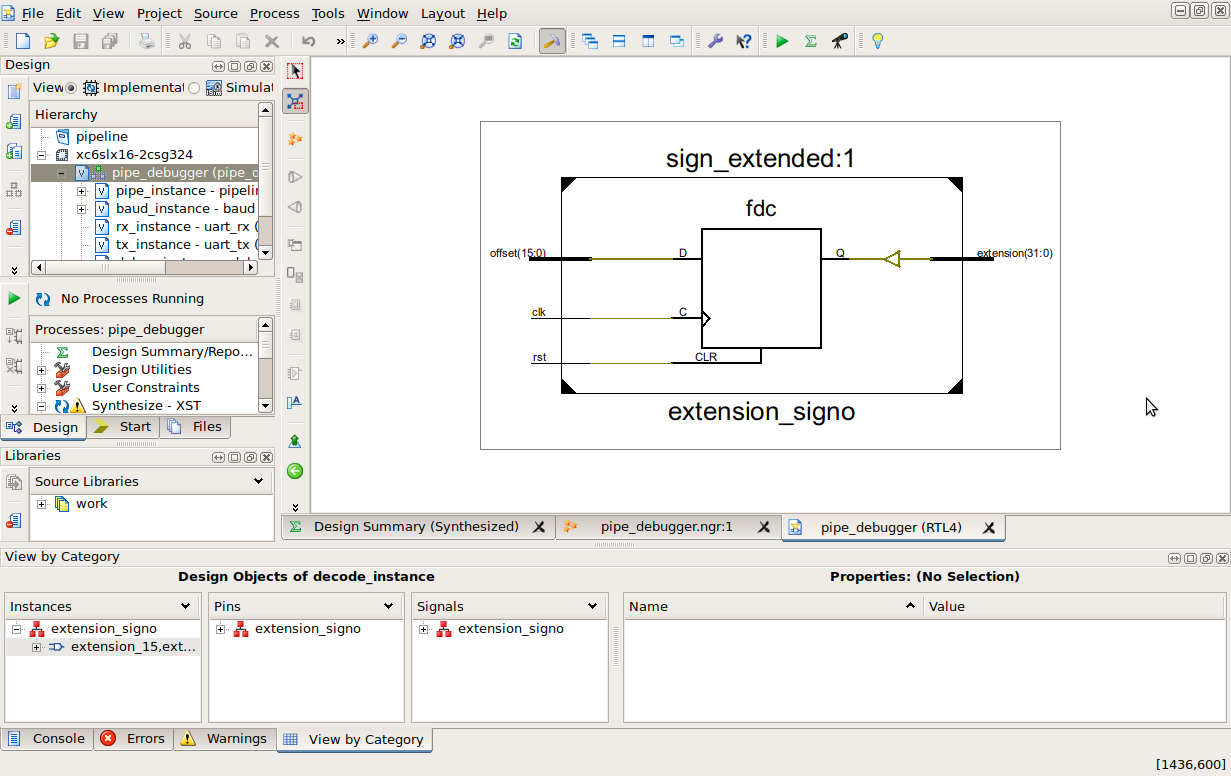
\includegraphics[scale=0.5]{img/extension_signo_inside}
\caption{Unidad de extensi\'on de signo}
\label{fig:sign_extended}
\end{figure}


\subsection{Multiplexor de stop}
Este m\'odulo se encarga, en caso de que la senal de stop est\'e activada, de rellenar con ceros el dato que sale de este modulo que son las senales que activan la unidad de control.

\begin{figure}[H]
\centering
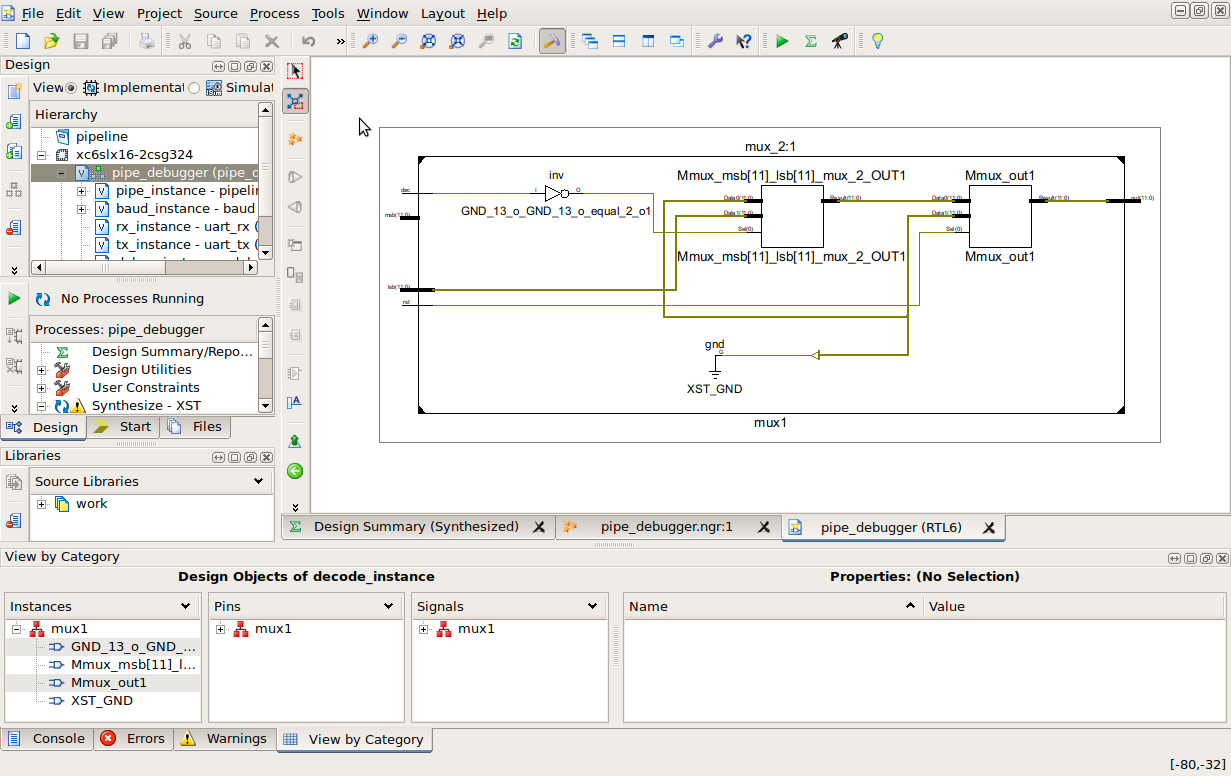
\includegraphics[scale=0.5]{img/multiplexor_inside}
\caption{Multiplexor de senales de la unidad de control}
\label{fig:sign_extended}
\end{figure}
